% !TeX root = ../main.tex
\graphicspath{{Figures/Methods}}

\chapter{Methods}\label{ch:methods}

\section{Data acquisition and catalogue formation}\label{methods:sec:data_agg}
This chapter comprehensively details the computational and statistical methods that were developed to produce an end-to-end machine learning pipeline for predicting drug resistance for M.tb and flaggin candidate variants to explain False Negative samples. Constructing a robust dataset for model-training and candidate variant identification, approximately $45,000$ M.tb genomes were downloaded from the Sequence Read Archives (SRA) and European Nucleotide Archive (ENA) repositories \cite{sra_infra_2022, ena_infra_2024}.

The methods is partitoned into $3$ phases. Firstly, an initial mapping is constructed using the WHO mutation catalogue \cite{WHOcatalog} and correspondingly updated with updated ``expert-rule'' heuristics. Secondly, a variant-discovering pipeline utilised identified FN samples to aggregate uncatalogued, highly significant variants. Thirdly, these variant features were supplied to a parallelised, single-layer neural network, designed to map sparse variant inputs directly to continuous, multi-drug probability outputs.

The remaining sections of this chapter follow the structure: Section 2.1 outlines data ingestion from the WHO-catalogue, Section 2.2 details rule-based variant filtering to updte the WHO-catalogue; and Section 2.3 defines the neural network parameters, custom loss functions, and post-training ablation study. 

\subsection{The WHO catalogue of mutations}
To construct features representing resistance-conferring variants from the WHO-catalogue of mutations, variant-feature mapping was done. The WHO catalogue MS Excel files were retrieved from the "mutation-catalogue-2023" repository \cite{WHOcatalog}. The variant features were constructed by forming a string of the variant position, reference allele and alternate allele(s): \texttt{POS\_REF\_ALT}. With the selected variants being restricted to ``Associated with Resistance'' or ``Associated with Resistance-interim'', the final confidence grade for each variant was limited to 1 or 2. A final confidence variant of $3$ meant ``Not Associated with Resistance'', and a grade of $4$ and $5$ meant ``Not Associated with Resistance-interim'' and ``Not Associated with Resistance'', respectively \cite{Walker2022, WHOcatalog} (Figure~\ref{fig:who}). Using these constraints, the catalogue was constructed into a map of 15 anti-TB drugs with their corresponding resistance-conferring variants.\\

\begin{figure}[H]
  \centering
   \begin{tabular}{|c|c|}
    \hline
    Group & Classification \\
    \arrayrulecolor{red}\hline
    1 & Assoc R \\
    \arrayrulecolor{red}\hline
    2 & Assoc w R-interim \\
    \arrayrulecolor{red}\hline
    3 & Uncertain significance \\
    \arrayrulecolor{black}\hline
    4 & Not assoc with R-interim \\
    \hline
    5 & Not assoc with R \\
    \hline
  \end{tabular}
  \\[1cm]
  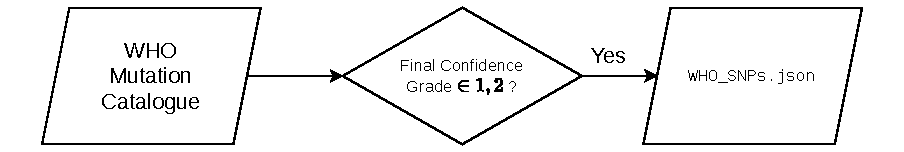
\includegraphics[width=\textwidth]{figures/who_snps.pdf}
  \caption{WHO SNP filtering process}
  \label{fig:who}
\end{figure}

\subsection{Updating the WHO catalogue with expert rules}
To update the WHO catalogue with ``expert rules'' released in the latest version \cite{WHOcatalog}, rule-based variant-filtering and variant-feature mapping was employed.

The WHO expert rules were acquired from the WHO-catalogue report released in 2023 \cite{WHOcatalog}. The expert-rules were implemented to extract variants from $\sim$45,000 M.tb VCF files. The M.tb VCF files were produced primarily from an alternative pipeline with variant-calling being done with Snippy \cite{tseemann_snippy} and variant annotation by SnpEff \cite{cingolani2012program}. The M.tb genomes were downloaded from the Sequence Read Archive (SRA) and ENA genome databases \cite{sra_infra_2022, ena_infra_2024}.

The expert rules that could be incorporated into the pipeline were rules 6–11, as the older rules involved processing MIC data or phenotypic measurements which were out of the scope for our project. Rule 6 stated any non-synonymous variant in the Rifampicin Resistance Determining Region (RRDR) of \textit{rpoB} (codons 426–452) were upgraded to final confidence grade (group) 2, meeting our criteria and thus, collected. Rule 7 collected variants for Fluoroquinolone (FQ) cross-resistance, any \textit{gyrA/gyrB} variant graded 1 or 2 for Levofloxacin (LFX) but 3 for Moxifloxacin (MFX), was upgraded to group 2 and vice versa. Rule 8 collected variants for Isoniazid-Ethionamide (INH-ETO) cross-resistance, where any \textit{inhA/fabG1} variant graded for INH but 3 for ETO cases was upgraded to 2 for the ETO and vice versa. Rule 9 collected variants for Bedaquiline-Clofazimine (BDQ-CFZ) cross-resistance, with any \textit{Rv0678/mmpL5} variants graded 1 or 2 for BDQ but group 3 for CFZ were upgraded to level 2 for CFZ. Rule 10 concerned pooling Loss-of-Function (LoF) variants in \textit{ddn, fbiA, fbiB, fbiC, fgd1, Rv2983} for Delamanid and Pretomanid DLM/PA. Rule 11 more broadly collected non-synonymous variants including LoF, earlyy stop, frameshift, gene deletion, or start-loss, in \textit{ethA, gid, katG, pncA, Rv0678, rpsA, ddn, fbiA, fbiB, fbiC, fgd1, Rv2983, tlyA}, were upgraded to group 2 for their respective drugs. Lastly from the previous version of expert-tules\cite{miotto2018}, any pncA variant was assumed to be resistant,  and correspondingly upgraded to group 1 or 2. Additionally, variants were harvested from intergenic regions aswell, with only synonymous variants  being skipped. Using the said expert rules, additional variants were harvested from $\sim$45,000 VCF files. Lastly, they were incorporated into the relevant drug index from WHO mapping.

\begin{figure}[htbp]
  \centering
  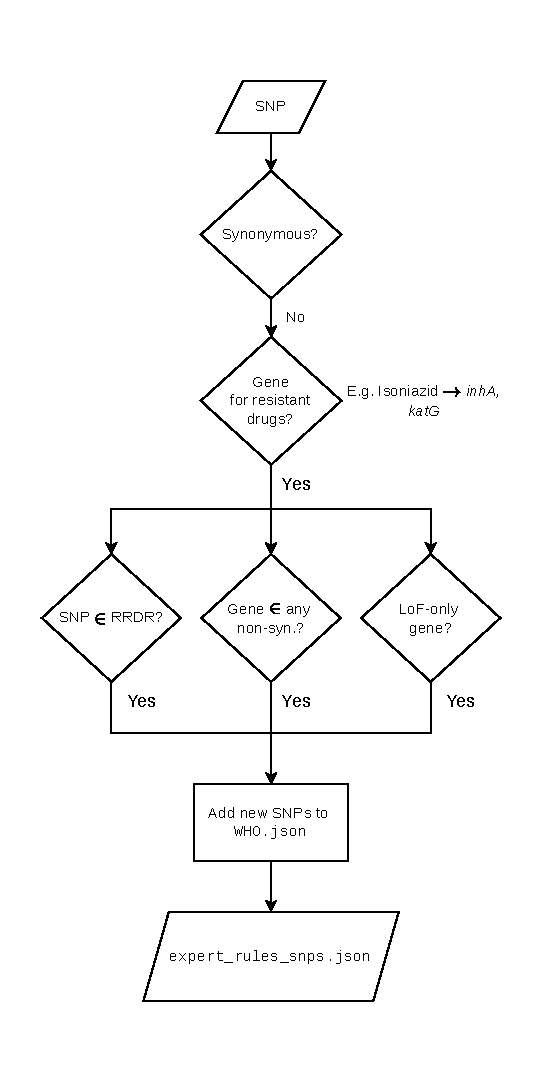
\includegraphics[width=1\textwidth]{figures/er.drawio-1.pdf}
  \caption{Expert rules SNP filtering process}
  \label{fig:er}
\end{figure}

\section{Augmenting updated catalogues}

\subsection{Resistance profiling and identification of False Negatives}
To identify False Negative (FN) samples for 22 anti-TB drugs, TB-Profiler (v6.6.6) \cite{phelan2019integrating} was use employed to profile over 45,000 M.tb genomes. 45,000 M.tb genomes were retrieved from the SRA and ENA databases \cite{sra_infra_2022, ena_infra_2024}. Of the 45,840 genomes retrieved, 45,702 were sequenced using short-read Illumina sequencing \cite{Bentley2008} and 138 were sequenced using Oxford Nanopore sequencing \cite{Jain2018}. Profiling for each sample was done with \texttt{tb-profiler predict} with parameters \texttt{--txt --no\_trim}. The mutation database used by TB-Profiler was version 2 of the WHO catalogue \texttt{WHO-v2-Strict} \cite{phelan2019integrating}. 

Resistance profiles produced from TB-Profiler were compared to phenotypic susceptibility data for at least 1 drug per sample. The confusion matrix was defined as follows:
\begin{itemize}
  \item \textbf{True Positive:} Both resistance-prediction and phenotype was Resistant.
  \item \textbf{False Negative:} The resistance-prediction was Susceptible, whereas the phenotype was Resistant. These files were our primary focus.
\item \textbf{True Negative:} Both resistance-prediction and phenotype were Susceptible.
\item \textbf{False Positive:} The resistance-prediction was Resistant, whereas the phenotype was Susceptible.
\end{itemize}

Using these classifications, we isolated samples that were FN for a particular drug (Figure~\ref{fig:filt}). 

\subsection{Identifying resistance-conferring candidate variants}
To augment the updated WHO catalogue map, for all variants identified in the FN samples, a Fishcer's Exact test was conducted. For 22 anti-TB agents, a $|\text{M.tb genomes}| \times |\text{Unique variants}|$, binary variant matrix was constructed. Using TN samples as a control, $p$-values (p-vals) and Odd Ratios (ORs) were calculated using the Fischer's Exact Test. To identify variants that were significant in the FN samples and associated with resistance, a filter of $-log_{10}(pval) \leq 5$ and $-log_{10}(OR) \> 1$ was imposed. Any p-value or OR that had a calculated value of \texttt{inf} or \texttt{-inf} were ignored.

To ensure the significant variants were not markers of M.tb lineage \cite{gagneux2018}, a variant was removed if it was in a list of identified lineage markers \cite{freschi2021population}. Lastly, if the variant was not already included in the updated WHO map, then the variant was added for that specific drug (Figure~\ref{fig:filt}) 


\begin{figure}[htbp]
  \centering
  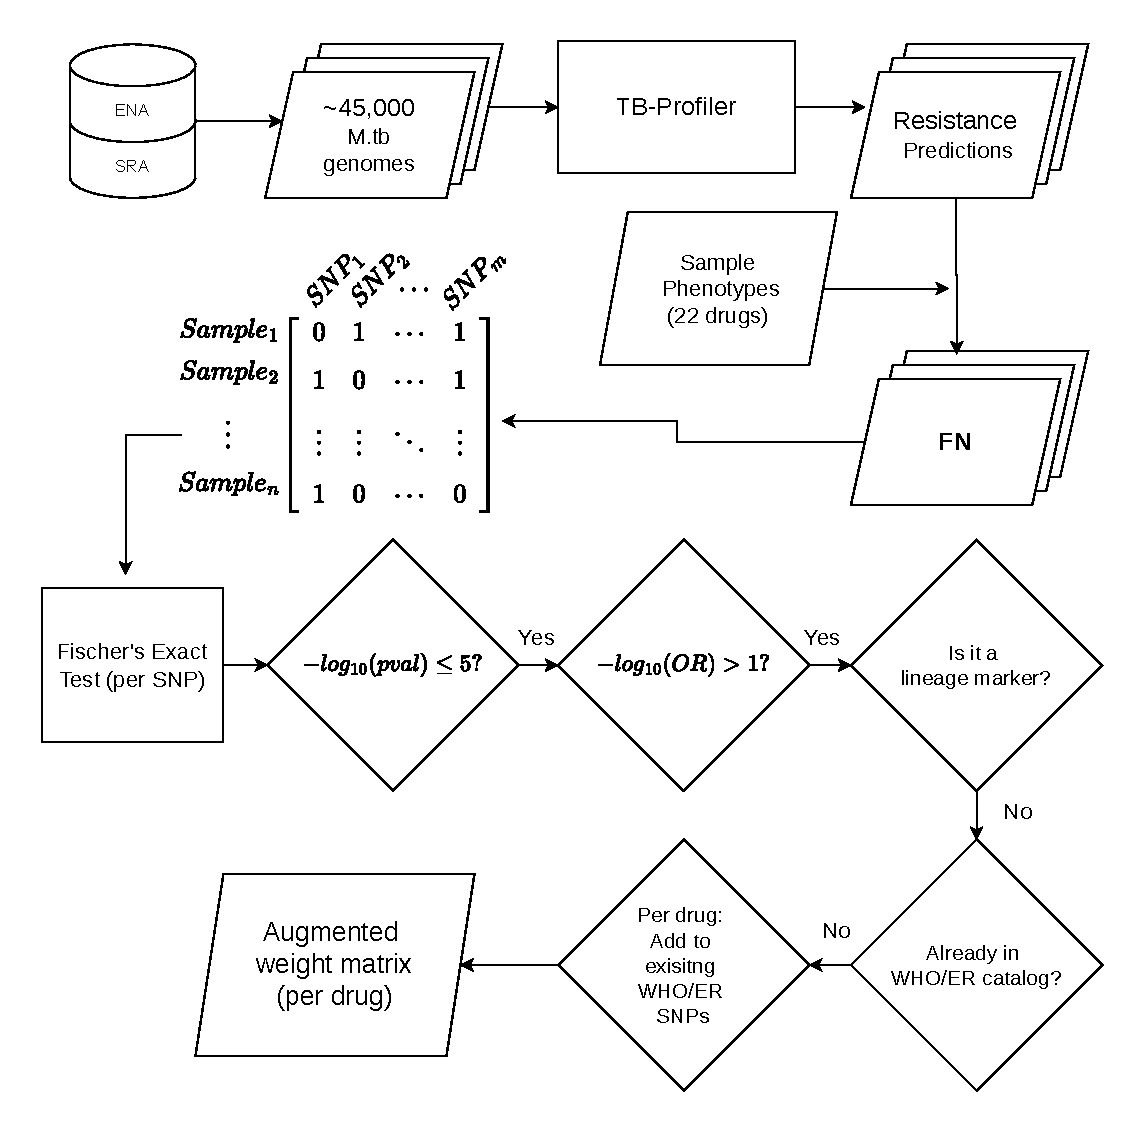
\includegraphics[width=1\textwidth]{figures/filt.drawio.pdf}
  \caption{Filtering SNP from FNs and augmented existing catalogues}
  \label{fig:filt}
\end{figure}

\section{Probabilistic implementation of a resistance prediction tool}

This section outlines the implementation and training framework of the parallelised, neural network built to provide a transition from rigid, static catalogue look-ups to a dynamic probabilistic method. Simulatenously, probabilities for 15 anti-TB drugs would be predicted. As shown in Figure~\ref{fig:train} the network adjusts weights based off a Loss function, which in this case was a customised Binary Cross-Entropy (BCE) A mask was implemented to ignore phenotypic data that was missing, ensuring proper training of the network. Following training, a threshold sweep was conducted to find prediction thresholds that maximised sensitivity, with a specificity constraint. Finally, an ablation study was conducted to quantify the impact of variants harvested from FNs had on the sensitivity.

This section is outlined as follows: Section 2.3.1 defined the layer connectivity matrices, weight scaling factors, and anchor regulariser equations; Section 2.3.2 describes data splitting criteria, strategies to address class imbalances, and a masked approach to gradient updates. Lastly, Section 2.3.3 estbalishes the threshold evlauation sweeps and feature ablation criteria.

\subsection{Network architecture and weights initisiatilisation}
To produce a resistance prediction for a sample, for a particular drug, a probability was produced a neuron with a sigmoid activation function. Firstly, the variant from a sample VCF was transformed into a binary input tensor $\mathbf{x} \in \{0,1\}^{26k\times1}$. If the sample contained a variant in the WHO map (with $\sim26k$ variants), then it was encoded by 1, 0, if not. The input tensor, $\mathbf{x}$ was passed into neuron that represents a particular drug. The weights for the neuron was set by the $n$ variants included for the drug in the WHO variant map. Those $n$ variants had an edge weight of 1 and the remaining $\sim26k-n $ variants were set to 0. Before training, the bias for the network was set to 0. Ultimately, the summation of inputs and weights $\mathbf{w}^{T}\mathbf{x}$,were passed into the sigmoid activation function, $$\sigma = \frac{1}{1+e^{-x}}$$ which produced a probability, $\hat{p} \in [0,1]$. A threshold of $\hat{p} > 0.5$ was applied for a resistance prediction (Figure~\ref{fig:onescheme}). 

\begin{figure}[htbp]
  \centering
  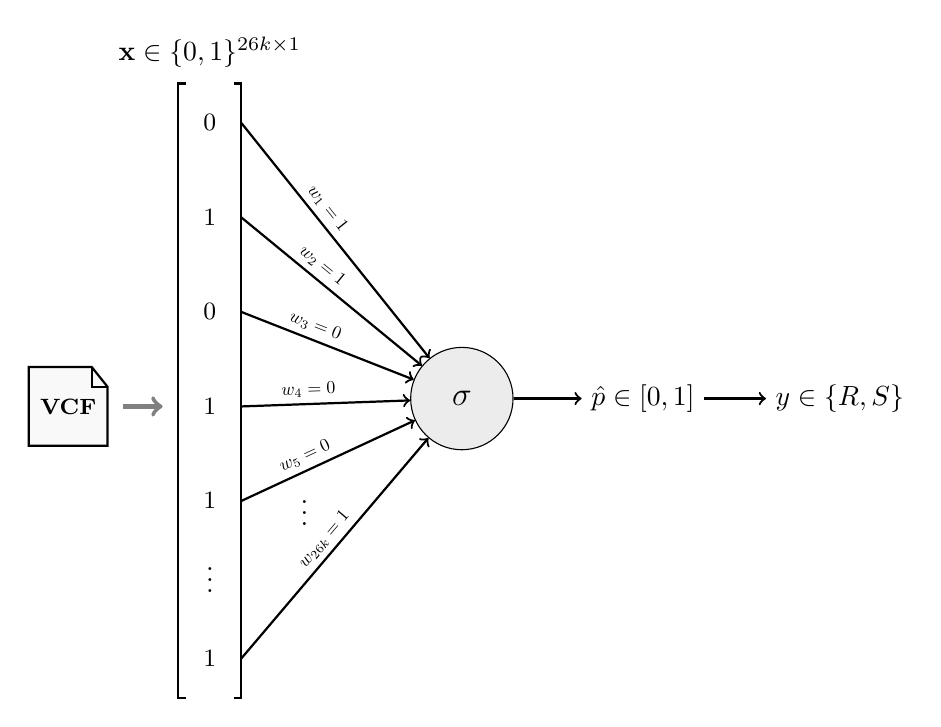
\begin{tikzpicture}[
      % Style for the binary digits inside the input vector
      input_node/.style={draw=none, minimum size=0.6cm, font=\small},
      % Style for the single MUCH LARGER Sigmoid processing node
      sigm_node/.style={circle, draw=black, minimum size=1.3cm, fill=gray!15, font=\large\bfseries},
      % Style for plain text/labels
      plain/.style={draw=none}
  ]

      % --- 0. VCF FILE ICON ---
      \draw[thick, fill=gray!5] (-2.3, 0.4) -- (-1.5, 0.4) -- (-1.3, 0.15) -- (-1.3, -0.6) -- (-2.3, -0.6) -- cycle;
      \draw[thick] (-1.5, 0.4) -- (-1.5, 0.15) -- (-1.3, 0.15);
      \node[font=\footnotesize\bfseries] at (-1.8, -0.1) {VCF};
      
      % Arrow from VCF file to Input Vector
      \draw[->, ultra thick, gray] (-1.1, -0.1) -- (-0.6, -0.1);


      % --- 1. INPUT LAYER (26k SNP Binary Vector) ---
      \draw[thick] (-0.3, 4.0) -- (-0.4, 4.0) -- (-0.4, -3.8) -- (-0.3, -3.8); 
      \draw[thick] (0.3, 4.0) -- (0.4, 4.0) -- (0.4, -3.8) -- (0.3, -3.8); 
      
      \node[plain] at (0, 4.4) {$\mathbf{x} \in \{0,1\}^{26k \times 1}$};

      % Binary Elements
      \node[input_node] (in1) at (0, 3.5)  {$0$};
      \node[input_node] (in2) at (0, 2.3)  {$1$};
      \node[input_node] (in3) at (0, 1.1)  {$0$};
      \node[input_node] (in4) at (0, -0.1) {$1$};
      \node[input_node] (in5) at (0, -1.3) {$1$};
      \node[plain]      (indot) at (0, -2.2) {$\vdots$};
      \node[input_node] (in26k) at (0, -3.3) {$1$};


      % --- 2. THE LARGE SIGMOID NEURON (Centered at Y=0) ---
      \node[sigm_node] (sig1) at (3.2, 0) {$\sigma$};


      % --- 3. SYNAPSE CONNECTIONS ---
      % All inputs converge cleanly into the large single neuron node
      \draw[->, thick] (0.4,3.5) -- node[above, pos=0.4, scale=0.65, sloped, black] {$w_1=1$} (sig1);
      \draw[->, thick] (0.4, 2.3) -- node[above, pos=0.4, scale=0.65, sloped, black] {$w_2=1$} (sig1);
      \draw[->, thick] (0.4, 1.1) -- node[above, pos=0.4, scale=0.65, sloped, black] {$w_3=0$} (sig1);
      \draw[->, thick] (0.4,-0.1) -- node[above, pos=0.4, scale=0.65, sloped, black] {$w_4=0$} (sig1);
      \draw[->, thick] (0.4, -1.3) -- node[above, pos=0.4, scale=0.65, sloped, black] {$w_5=0$} (sig1);
      \node[plain] (dot) at (1.2,-1.35) {$\vdots$};
      \draw[->, thick] (0.4, -3.3) -- node[above, pos=0.5, scale=0.65, sloped, black] {$w_{26k}=1$} (sig1);



      % --- 4. INTERMEDIATE LAYER (Scalar Probability Output) ---
      \node[plain] (p1) at (5.5, 0) {$\hat{p} \in [0,1]$};
      \draw[->, thick] (sig1) -- (p1);

      % --- 6. OUTPUT LAYER (Final Single Drug Susceptibility Class) ---
      \node[plain] (y1) at (8, 0) {$y \in \{R, S\}$};
      \draw[->, thick] (p1) -- (y1);

  \end{tikzpicture}
  \caption{Schematic for one neuron with weights specified for a particular drug}
  \label{fig:onescheme}
\end{figure}

For all 15 anti-TB drugs from the WHO catalogue, 15 neurons corresponding to each drug produced an output vector $\mathbf{y}\in {R,S}^{15\times1}$ (Figure~\ref{fig:fullschem}).

\begin{figure}
  \centering
  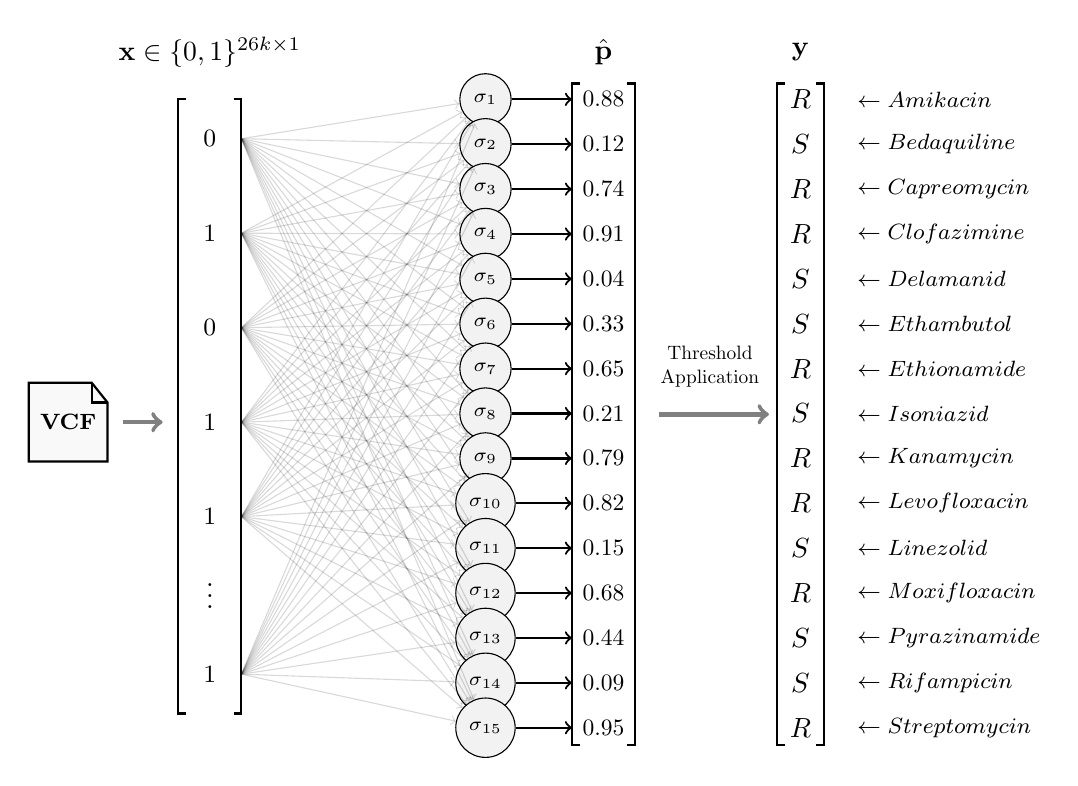
\begin{tikzpicture}[
      % Style for the binary digits inside the input vector
      input_node/.style={draw=none, minimum size=0.6cm, font=\small},
      % Style for the 15 Sigmoid processing nodes
      sigm_node/.style={circle, draw=black, minimum size=0.65cm, fill=gray!10, font=\scriptsize},
      % Style for plain text/labels
      plain/.style={draw=none},
      % Custom style to draw a document/file icon
      file_icon/.style={
          draw, thick, fill=white,
          append after command={
              % Draws the folded corner of the paper icon
              [shift={(-0.15,-0.2)}] (\numexpr\tikzlastnode\relax.north east) -- 
              ++(-0.25,0) -- ++(0,0.25) -- cycle
          }
      }
  ]

      % --- 0. VCF FILE ICON (Shifted right from -3.3 to -1.8) ---
      \draw[thick, fill=gray!5] (-2.3, 0.4) -- (-1.5, 0.4) -- (-1.3, 0.15) -- (-1.3, -0.6) -- (-2.3, -0.6) -- cycle;
      \draw[thick] (-1.5, 0.4) -- (-1.5, 0.15) -- (-1.3, 0.15);
      \node[font=\footnotesize\bfseries] at (-1.8, -0.1) {VCF};
      
      % Shorter Arrow from VCF file to Input Vector
      \draw[->, ultra thick, gray] (-1.1, -0.1) -- (-0.6, -0.1);


      % --- 1. INPUT LAYER (26k SNP Binary Vector) ---
      % Vector Brackets
      \draw[thick] (-0.3, 4.0) -- (-0.4, 4.0) -- (-0.4, -3.8) -- (-0.3, -3.8); 
      \draw[thick] (0.3, 4.0) -- (0.4, 4.0) -- (0.4, -3.8) -- (0.3, -3.8); 
      
      \node[plain] at (0, 4.6) {$\mathbf{x} \in \{0,1\}^{26k \times 1}$};

      % Binary Elements
      \node[input_node] (in1) at (0, 3.5)  {$0$};
      \node[input_node] (in2) at (0, 2.3)  {$1$};
      \node[input_node] (in3) at (0, 1.1)  {$0$};
      \node[input_node] (in4) at (0, -0.1) {$1$};
      \node[input_node] (in5) at (0, -1.3) {$1$};
      \node[plain]      (indot) at (0, -2.2) {$\vdots$};
      \node[input_node] (in26k) at (0, -3.3) {$1$};


      % --- 2. 15 SIGMOID NODES LAYER ---
      \foreach \j in {1,...,15} {
          \pgfmathsetmacro{\ypos}{4.0 - (\j-1) * 0.57}
          \node[sigm_node] (sig\j) at (3.5, \ypos) {$\sigma_{\j}$};
      }


      % --- 3. DENSE SYNAPSE CONNECTIONS ---
      \foreach \j in {1,...,15} {
          \draw[->, thin, opacity=0.15] (0.4,3.5) -- (sig\j);
          \draw[->, thin, opacity=0.15] (0.4, 2.3) -- (sig\j);
          \draw[->, thin, opacity=0.15] (0.4, 1.1) -- (sig\j);
          \draw[->, thin, opacity=0.15] (0.4, -0.1) -- (sig\j);
          \draw[->, thin, opacity=0.15] (0.4, -1.3) -- (sig\j);
          \draw[->, thin, opacity=0.15] (0.4, -3.3) -- (sig\j);
      }


      % --- 4. INTERMEDIATE LAYER (Probability Vector shifted left to X=5.0) ---
      \foreach \j / \prob in {
          1/0.88, 2/0.12, 3/0.74, 4/0.91, 5/0.04, 
          6/0.33, 7/0.65, 8/0.21, 9/0.79, 10/0.82, 
          11/0.15, 12/0.68, 13/0.44, 14/0.09, 15/0.95
      } {
          \pgfmathsetmacro{\ypos}{4.0 - (\j-1) * 0.57}
          \node[plain] (p\j) at (5.0, \ypos) {\scalebox{0.85}{$\prob$}};
          % Shorter line endpoint target changed to 4.6
          \draw[->, thick] (sig\j) -- (4.6, \ypos);
      }
      
      % Probability Vector Brackets (Shifted to encompass X=5.0)
      \draw[thick] (4.7, 4.2) -- (4.6, 4.2) -- (4.6, -4.2) -- (4.7, -4.2); 
      \draw[thick] (5.3, 4.2) -- (5.4, 4.2) -- (5.4, -4.2) -- (5.3, -4.2); 
      \node[plain] at (5.0, 4.6) {$\hat{\mathbf{p}}$};


      % --- 5. THRESHOLD APPLICATION TRANSITION (Compensated leftward shift) ---
      \draw[->, ultra thick, gray] (5.7, 0) -- node[above, black, align=center, scale=0.7, yshift=10pt, xshift=-2pt] {Threshold\\Application} (7.1, 0);


      % --- 6. OUTPUT LAYER (Final Vector shifted left to X=7.5) ---
      \foreach \j / \res / \drug in {
          1/R/Amikacin, 2/S/Bedaquiline, 3/R/Capreomycin, 4/R/Clofazimine, 
          5/S/Delamanid, 6/S/Ethambutol, 7/R/Ethionamide, 8/S/Isoniazid, 
          9/R/Kanamycin, 10/R/Levofloxacin, 11/S/Linezolid, 12/R/Moxifloxacin, 
          13/S/Pyrazinamide, 14/S/Rifampicin, 15/R/Streptomycin
      } {
          \pgfmathsetmacro{\ypos}{4.0 - (\j-1) * 0.57}
          
          % Final categorical value
          \node[plain] (y\j) at (7.5, \ypos) {$\text{\res}$};
          
          % Right Annotation (Drug Names shifted closer)
          \node[plain, anchor=west, font=\footnotesize] at (8.1, \ypos) {$\leftarrow \text{\drug}$};
      }

      % Final Classification Vector Brackets (Shifted to encompass X=7.5)
      \draw[thick] (7.3, 4.2) -- (7.2, 4.2) -- (7.2, -4.2) -- (7.3, -4.2); 
      \draw[thick] (7.7, 4.2) -- (7.8, 4.2) -- (7.8, -4.2) -- (7.7, -4.2); 

      \node[plain] at (7.5, 4.6) {$\mathbf{y}$};

  \end{tikzpicture}
  \caption{Neural Net schematic for 15 drugs}
  \label{fig:fullschem}
\end{figure}


\subsection{Training regime and optimisation}
To provide an alternative to rigid look-up mechanics of a catalogue and to capture continuous probabilistic thresholds for multi-drug resistance, a single-layer parallelised neural network was implemented in Tensorflow/Keras. Using this, complex multi-drug weights can be learned from $\sim$45,000 M.tb genomes.

The input layer accepts a high-dimensional, sparse feature tensor $x \in \{0,1\}^{N\times M}$, where $N$ represents the $\sim45,000$ M.tb genomes and $M$ represents the approximately 26,000 distinct variants compiled from the WHO-catalogue. $M > 26,000$ if the expert-rules variants and augmented variants were included. This feature matrix maps directly via a single dense hidden layer to a classification column vector $\hat{p}\in \{0,1\}^{15\times 1}$, where each row stores an independent resistance-prediction across 15 anti-TB drugs. 

The raw linear transformation logits $z$ are evlauated through an element-wise sigmoid activation function: $$ \hat{p}_i = \sigma(z_i) = \frac{1}{1+e^{-z_i}}$$

Rather than implementing a naive weight initisiatilisation strategy, the WHO-catalogue mutation knowledge was transferred. Baseline weight matrices ($W_{init}$) were pre-loaded from the WHO map formation. To optimise training convergence and push the network's boundaries closer to binary classification limits, the kernels scaled by a factor of $10.0$, and all corresponding node biases ($b$) were uniformly preset to a baseline constraint of $-5.0$: $$ W = W_{init}\times 10.0, b_i=-5.0 $$

To ensure the network retains it's biological anchor and avoids extreme weight drift during gradient updates, a custom anchor kernel regulariser was embedded within the loss-layer, penalising squared deviations from the initial configuration using a loss multiplier ($\lambda = 1 \times 10^{-5}$): $$ \Omega(W) = \lambda\sum_{j}(W_j - W_{init,j})^2$$

For efficient network parameter optimisation, while maintaining high predictive stability across highly imbalanced label streams, custom masking was employed. The input matrix, $x$, was split randomly into a $80:20$ train-test split (seeded at \texttt{random\_state=42}). For monitoring training validation and prevent over-fitting, the training set was further split into a manual $80:20$ train-validation configuration. The model was trained over $50$ epochs utilising the AdamW optimiser with a base learning rate ($\alpha$) of $1\times 10^{-3}$, and a batch size of $64$. Training was managed using an automated learning rate decay loop ($\texttt{ReduceLROnPlateau}$, decay factor = $0.2$, patience = $3$ epochs).

Since the phenotypic data for each sample included resistance data for at least one anti-TB drug (out of $22$), many samples had missing values for numerous drugs. Therefore a custom Masked Weigthed Binary Cross-Entropy (BCE) loss function was implemented. This function masked missing phenotypic data ($y_{ij}=\text{NaN}$) during backpropagation to prevent gradients from skewing. In the case of severe class imbalances, where the number of suscptible samples vastly outnumbered resistant samples, positive sample weights were adaptively regularised using the square root of the inverse class ratio calculated from the portion actively being trained: $$ w_{pos,i} = \sqrt{\frac{N_{\text{suscptible},i}}{N_{\text{resistant},i}+10^{-8}}} $$
$$\mathcal{L}_{\text{Masked}} =\frac{\sum_{i=1}^{15} m_i \cdot [w_{\text{pos},i} \cdot y_i log(\hat{p}_i)+(1-y_i)log(1-\hat{p}_i)]}{\sum_{i=1}^15 m_i + 10^{-8}}$$
Where $m_i \in \{0,1\}$ is a binary filter mask, where $m_i=1$ if phenotypic data is present, and $m_i=0$ if absent. 

Following training, the raw prediction vector was processed through a threshold sweep to determine the optimal threshold to predict resitance for that drug. Rather than the inflexible default cutoff ($0.5$), thresholds were dynamically set using receiver operating characteristic (ROC) curves. The threshold that maximised the sensitivity, whilst not degrading the specificity below a pre-defined threshold ($0.80$) were kept. 

Following threshold assignment for each drug, an \textit{in silico} feature ablation assay was conducted. This determined the drop in sensitivity by ablating the specific variant. The variant that were considered for ablation were the significant variants harvested from FN samples, in order to determine the loss of sensitivity caused by their exclusion. Systematically, variant features were excluded by zeroing out their respective index within the input tensor ($W_{\text{ablated}[\text{idx,}d]} = 0.0$). A variant was flagged to cause a significant change in sensitivity if it's exclusion resulted in a sensitivity drop of $\geq 0.05\%$ compared to the unablated baseline sensitivity.

\begin{figure}[htbp]
  \centering
  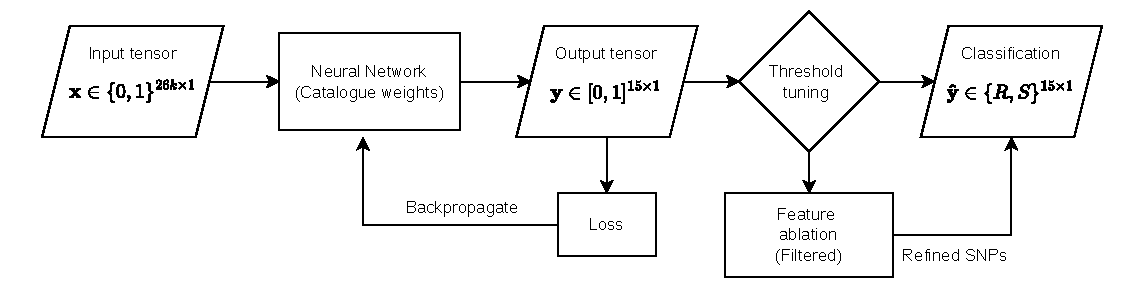
\includegraphics[width=1.2\textwidth]{figures/train.drawio.pdf}
  \caption{Training process}
  \label{fig:train}
\end{figure}

Summarising, the computational and statistical framework in this chapter outlines a pipeline designed to predict the resistance profile for an M.tb sample using an augmented version of the WHO-catalogue. Furthermore, in the process of augmenting the WHO-catalogue using significant variants, candidate variants that can account for the prediction-phenotype discordance in FN samples can be established, given wet-lab validation. The computational performance, validation evlauations, and maps of rescued candidate variants resulting from this pipeline is presented and analysed in Chapter 3.
